\documentclass{my-article}
\usepackage{my-coverpage}
\usepackage{my-codespace}

\usepackage[utf8]{inputenc}
\usepackage[T5]{fontenc}
\usepackage[vietnamese]{babel}

\usepackage{textcomp}
% =========================
% Cover page information
% =========================

\NameUpperUniname{Vietnam National University Ho Chi Minh City}
\NameUniname{Ho Chi Minh City University of Technology}
\NameDeptname{Faculty of Electrical and Electronics Engineering}
\NamePathlogo{./my-chapters/my-images/01_logobachkhoatoi.png}
\NameClass{Digital System Design \\ &  and Verification (EE3213)}
\NameGroup{04}
\NameLesson[\Large]{HOMEWORK REPORT}
\NameTitle[\Huge]{Chương 3 - Thiết kế mạch tổ hợp}
\NameAdvisor{Nguyễn Trung Hiếu}
\NamePlace{Ho Chi Minh}
\NameTime{../../20..}
\NamePathBackground[width=\paperwidth,height=\paperheight]{./my-chapters/my-images/bia.jpg} 
\MemberTableData{
1 & 2213874 & Nguyễn Thanh Tùng & L01 \\ \hline
2 & 2210780 & Nguyễn Đại Đồng & L01 \\ \hline
3 & 2213496 & Nguyễn Quốc Tín & L01 \\ \hline
}

% =========================
% Configuration
% =========================
%--- Header and footer
\fancyhf{}
\fancyhead[L]{\leftmark}
% =========================
% Document
% =========================

\newcommand{\question}[1]{%
	\section*{#1}%
	\addcontentsline{toc}{section}{#1}%
}
\newcommand{\answer}[2]{%
	\subsection*{\textbf{#1}\kern0.2em)~#2}%
	\addcontentsline{toc}{subsection}{#1)}%
}

\newcommand{\finalresult}[1]{%
	\begin{tikzpicture}[baseline=(content.base)]
		\node[draw=red, thick, rounded corners=3pt, inner sep=6pt] (content)
		{\ensuremath{#1}};
	\end{tikzpicture}%
}

\begin{document}
\pagestyle{empty}
\MycoverFinalProject % Cover page
\newpage
\renewcommand{\arraystretch}{1.5} % tăng khoảng cách dòng (row height)
\setlength{\parindent}{1cm}
\onehalfspacing
\setlength{\parskip}{6pt} 
\tableofcontents
\listoffigures
\listoftables
\listoflistings
\newpage
\pagestyle{fancy}
\MycountPages{number}
\fancyhead[R]{GVHD: Nguyễn Trung Hiếu}
\fancyfoot[L]{
\includegraphics[width=.02\linewidth]{./my-chapters/my-images/logo_DEE.png}\text{ Department of Electronics}}

\question{Câu 2}

Thiết kế mạch tổ hợp tìm vị trí bit 1 đầu tiên (tính từ MSB) của chuỗi 24-bit. Cho các standard cell như sau: cổng not, các cổng logic 2 ngõ vào, mux 2-1, mux 4-1.

\answer{a}{Thiết kế mạch chỉ được dùng các standard cell trên.}

Đầu tiên nhóm em sẽ thiết kế từ một bộ tìm kiếm vị trí bit 1 đầu tiên (tính từ MSB) cho một chuỗi 4-bit trước. 

\begin{table}[H]
	\centering
	\begin{tabular}{|c|c|c|c|c|c|c|}
		\hline
		\multicolumn{4}{|c|}{Input} & \multicolumn{2}{c|}{Output} & Zero Flag \\
		\hline
		$X_{3}$ & $X_{2}$ & $X_{1}$ & $X_{0}$ & $Y_{1}$ & $Y_{0}$ & $V$ \\
		\hline
		0 & 0 & 0 & 0 & 0 & 0 & 1 \\
		\hline
		0 & 0 & 0 & 1 & 0 & 0 & 0 \\
		\hline
		0 & 0 & 1 & X & 0 & 1 & 0 \\
		\hline
		0 & 1 & X & X & 1 & 0 & 0 \\
		\hline
		1 & X & X & X & 1 & 1 & 0 \\
		\hline
	\end{tabular}
	\caption{Bảng sự thật của bộ phát hiện bit 1 (Leading one position) cho 4 bit.}
	\label{tab:leading-one-4bit}
\end{table}

Từ bảng \ref{tab:leading-one-4bit}, ta rút gọn và có được mạch như sau:

\begin{figure}[H]
	\centering
	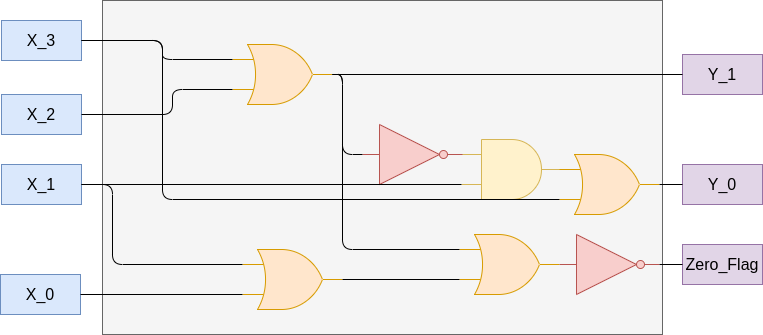
\includegraphics[width=.8\linewidth]{/home/noname/Documents/project_tiny/Ex3/20_doc/my-chapters/my-diagrams/Question2/spec.png}
	\caption{Sơ đồ logic của bộ LOPD 4bit.}
\end{figure}

Từ bộ LOPD 4-bit trên, ta triển khai bộ LOPD 8-bit và bộ LOPD 16-bit như sau:

\begin{figure}[H]
	\centering
	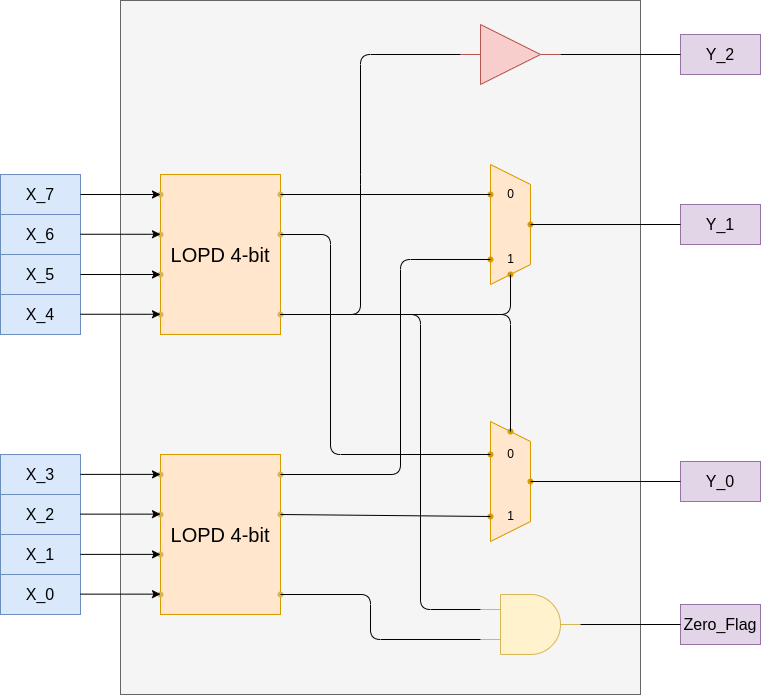
\includegraphics[width=.8\linewidth]{/home/noname/Documents/project_tiny/Ex3/20_doc/my-chapters/my-diagrams/Question2/LOPD_8bit.png}
	\caption{Sơ đồ logic của bộ LOPD 8bit.}
\end{figure}

\begin{figure}[H]
	\centering
	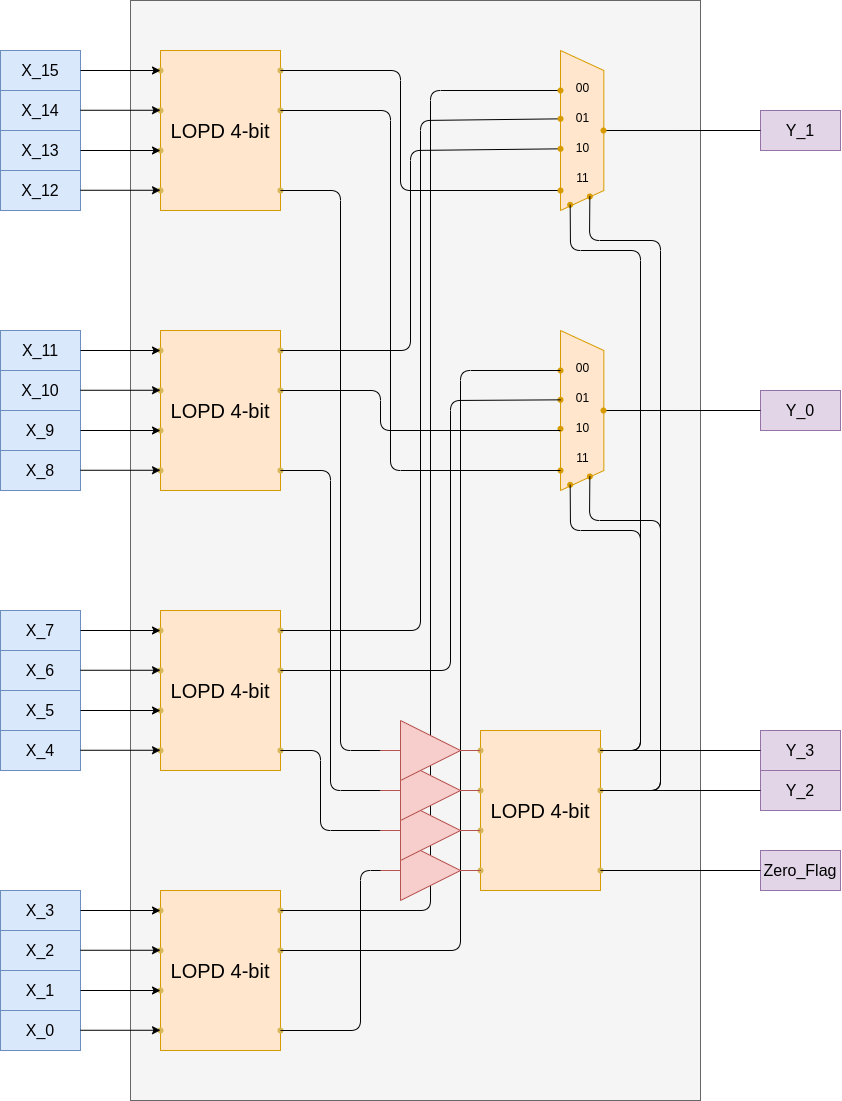
\includegraphics[width=.8\linewidth]{/home/noname/Documents/project_tiny/Ex3/20_doc/my-chapters/my-diagrams/Question2/LOPD_16bit.png}
	\caption{Sơ đồ logic của bộ LOPD 16bit.}
\end{figure}

Từ bộ LOPD 8-bit và LOPD 16-bit trên, ta ghép lại thành 24-bit với LOPD 8-bit vào vị trí 8-bit cao (từ $ 23 \rightarrow 16 $) và bộ LOPD 16-bit vào 16-bit thấp (từ $ 15 \rightarrow 0 $).

\begin{figure}[H]
	\centering
	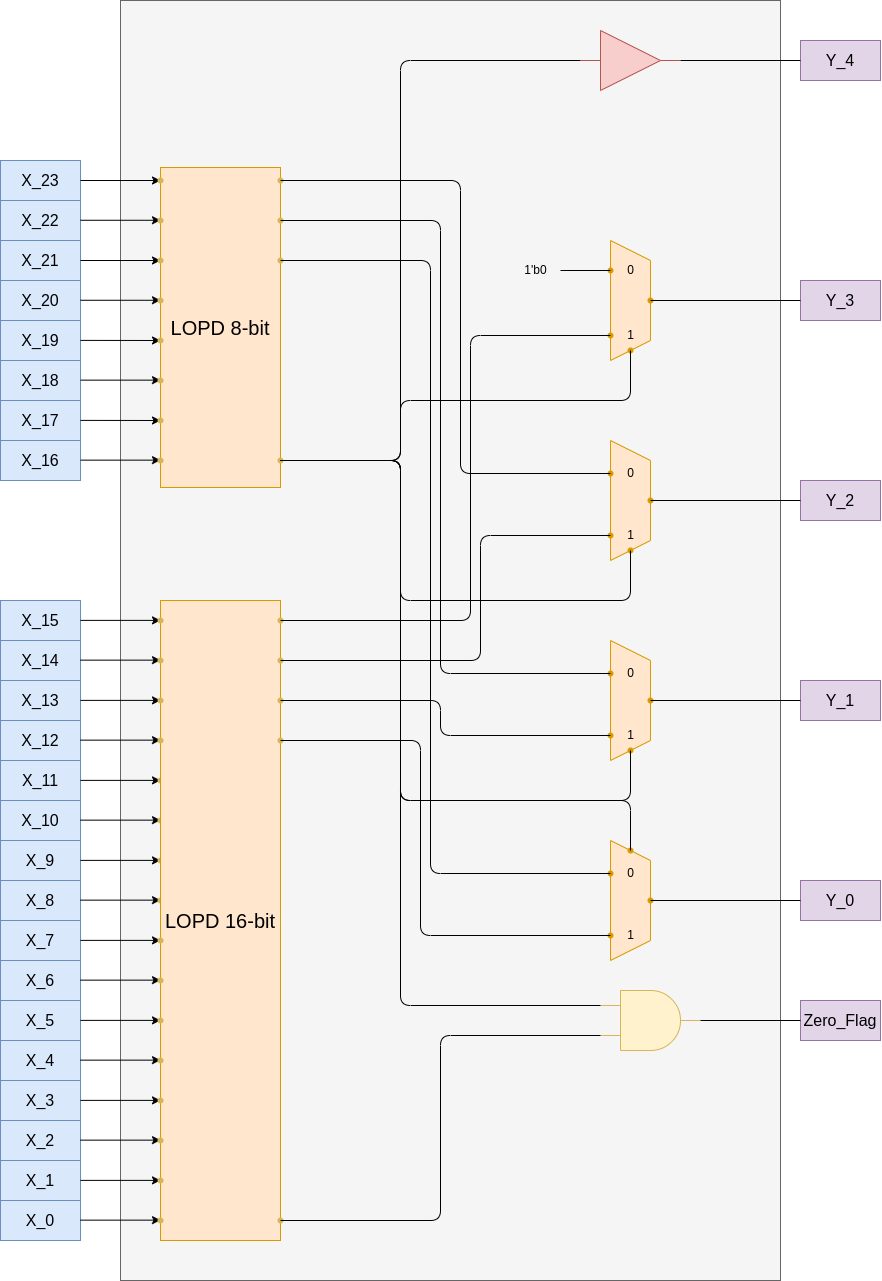
\includegraphics[width=.8\linewidth]{/home/noname/Documents/project_tiny/Ex3/20_doc/my-chapters/my-diagrams/Question2/LOPD_24bit.png}
	\caption{Sơ đồ logic của bộ LOPD 24-bit.}
\end{figure}

\answer{b}{Viết chương trình HDL mô tả mạch đã cho.}

\lstinputlisting[style=StyleCode, language=SystemVerilog, caption={Chương trình mô tả LOPD 4-bit.}]{/home/noname/Documents/project_tiny/Ex3/02_rtl/Question2/LOPD_4bit.sv}

\lstinputlisting[style=StyleCode, language=SystemVerilog, caption={Chương trình mô tả LOPD 8-bit.}]{/home/noname/Documents/project_tiny/Ex3/02_rtl/Question2/LOPD_8bit.sv}

\lstinputlisting[style=StyleCode, language=SystemVerilog, caption={Chương trình mô tả LOPD 16-bit.}]{/home/noname/Documents/project_tiny/Ex3/02_rtl/Question2/LOPD_16bit.sv}

\lstinputlisting[style=StyleCode, language=SystemVerilog, caption={Chương trình mô tả LOPD 24-bit.}]{/home/noname/Documents/project_tiny/Ex3/02_rtl/Question2/Question2.sv}

\answer{c}{Viết testbench cho mạch, thực hiện testbench với 100 mẫu và tính scoreboard của 100 mẫu đó.}

Đầu tiên nhóm em thưc hiện triển khai chứng minh kết quả đúng bằng giải thuật sau:

\begin{lstlisting}[style=StyleCode, language=SystemVerilog, caption={Giải thuật chứng minh kết quả của bộ LOPD 24-bit.}]
	function automatic logic [SIZE_LOP-1:0] Test_LOPD(
		input logic [SIZE_DATA-1:0]     f_i_data
	);
		logic [SIZE_DATA-1:0] t_temp;
		int cnt_position_1;
		begin
			t_temp = f_i_data;
			cnt_position_1 = 0;
			
			if(t_temp == 0) begin
				Test_LOPD = 0;
			end else begin
				while (t_temp[SIZE_DATA-1] == 0) begin
					t_temp = t_temp << 1;
					cnt_position_1 ++;
				end
				Test_LOPD = SIZE_DATA - cnt_position_1 - 1;
			end
		end
	endfunction
\end{lstlisting}


\question{Câu 6}

Thiết kế một bộ sắp xếp song song như hình dưới, mô tả giải thuật sắp xếp 8 mẫu ngõ vào $x_{1}$, $x_{2}$,$\dots, x_{8}$, và cho ngõ ra là $y_{1}$, $y_{2}$, $\dots, y_{8}$ theo thứ tự giảm dần (hoặc tăng dần).

\begin{figure}[H]
	\centering
	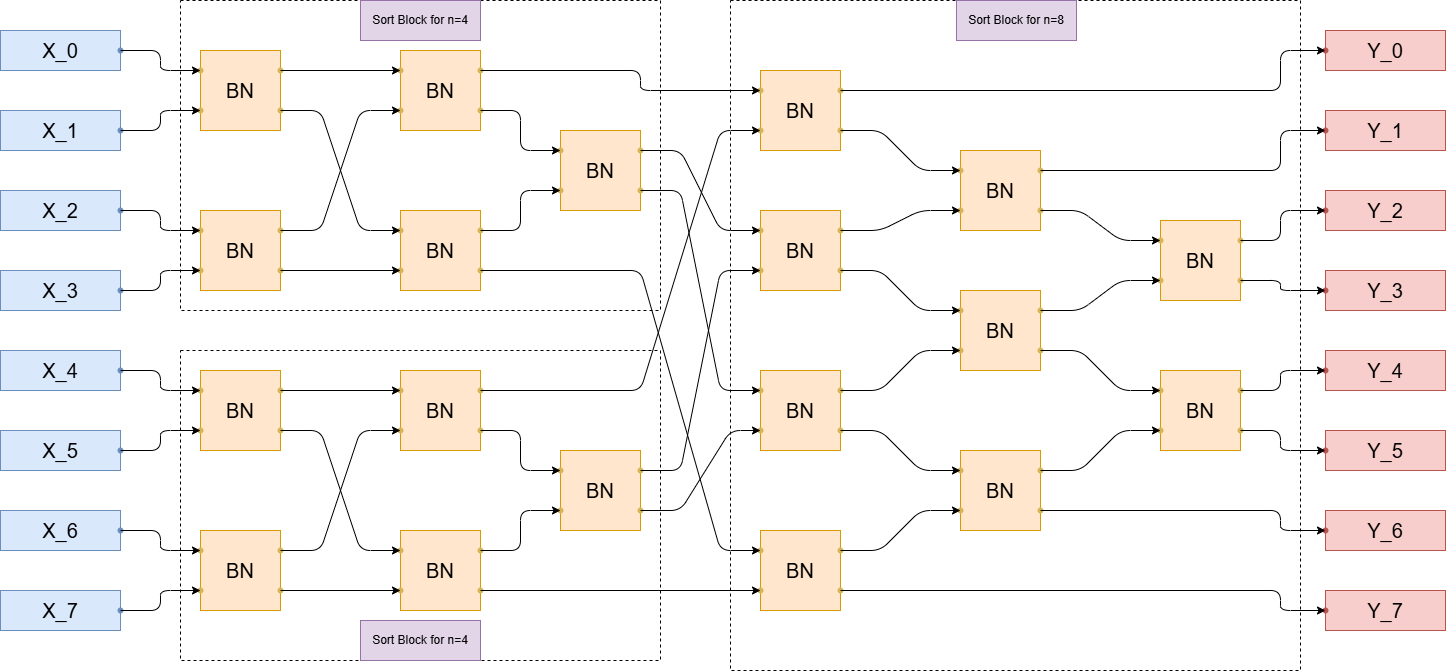
\includegraphics[width=\linewidth]{./my-chapters/my-diagrams/Question6/debai.png}
\end{figure}

Trong đó, mỗi bộ BN (Bitonic Sort) có cấu trúc như hình:

\begin{figure}[H]
	\centering
	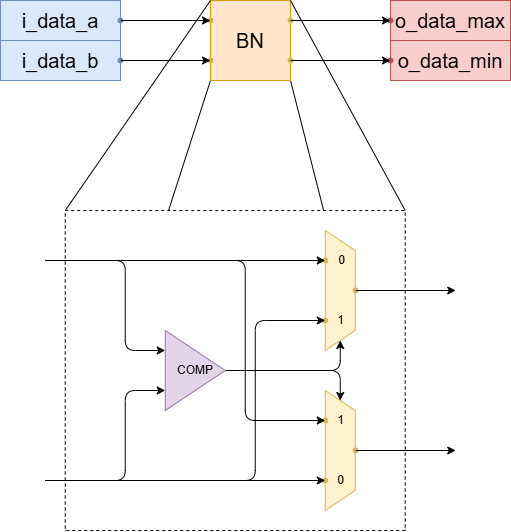
\includegraphics[width=.4z\linewidth]{./my-chapters/my-diagrams/Question6/Swap_and_compare.png}
\end{figure}

Cho các standard cell là: Cổng NOT, các cổng logic 2 ngõ vào, Mux 2-1, Mux 4-1.
\end{document}
